\section*{Anhang}
\addcontentsline{toc}{section}{Anhang}

\subsection*{Technische Umsetzung des UAP-Generierungsprozesses}

Die technische Umsetzung des Prozesses zur Generierung der \acrshort{uap} Bilder ist in der folgenden Grafik dargestellt:

\begin{figure}[H]
    \centering
    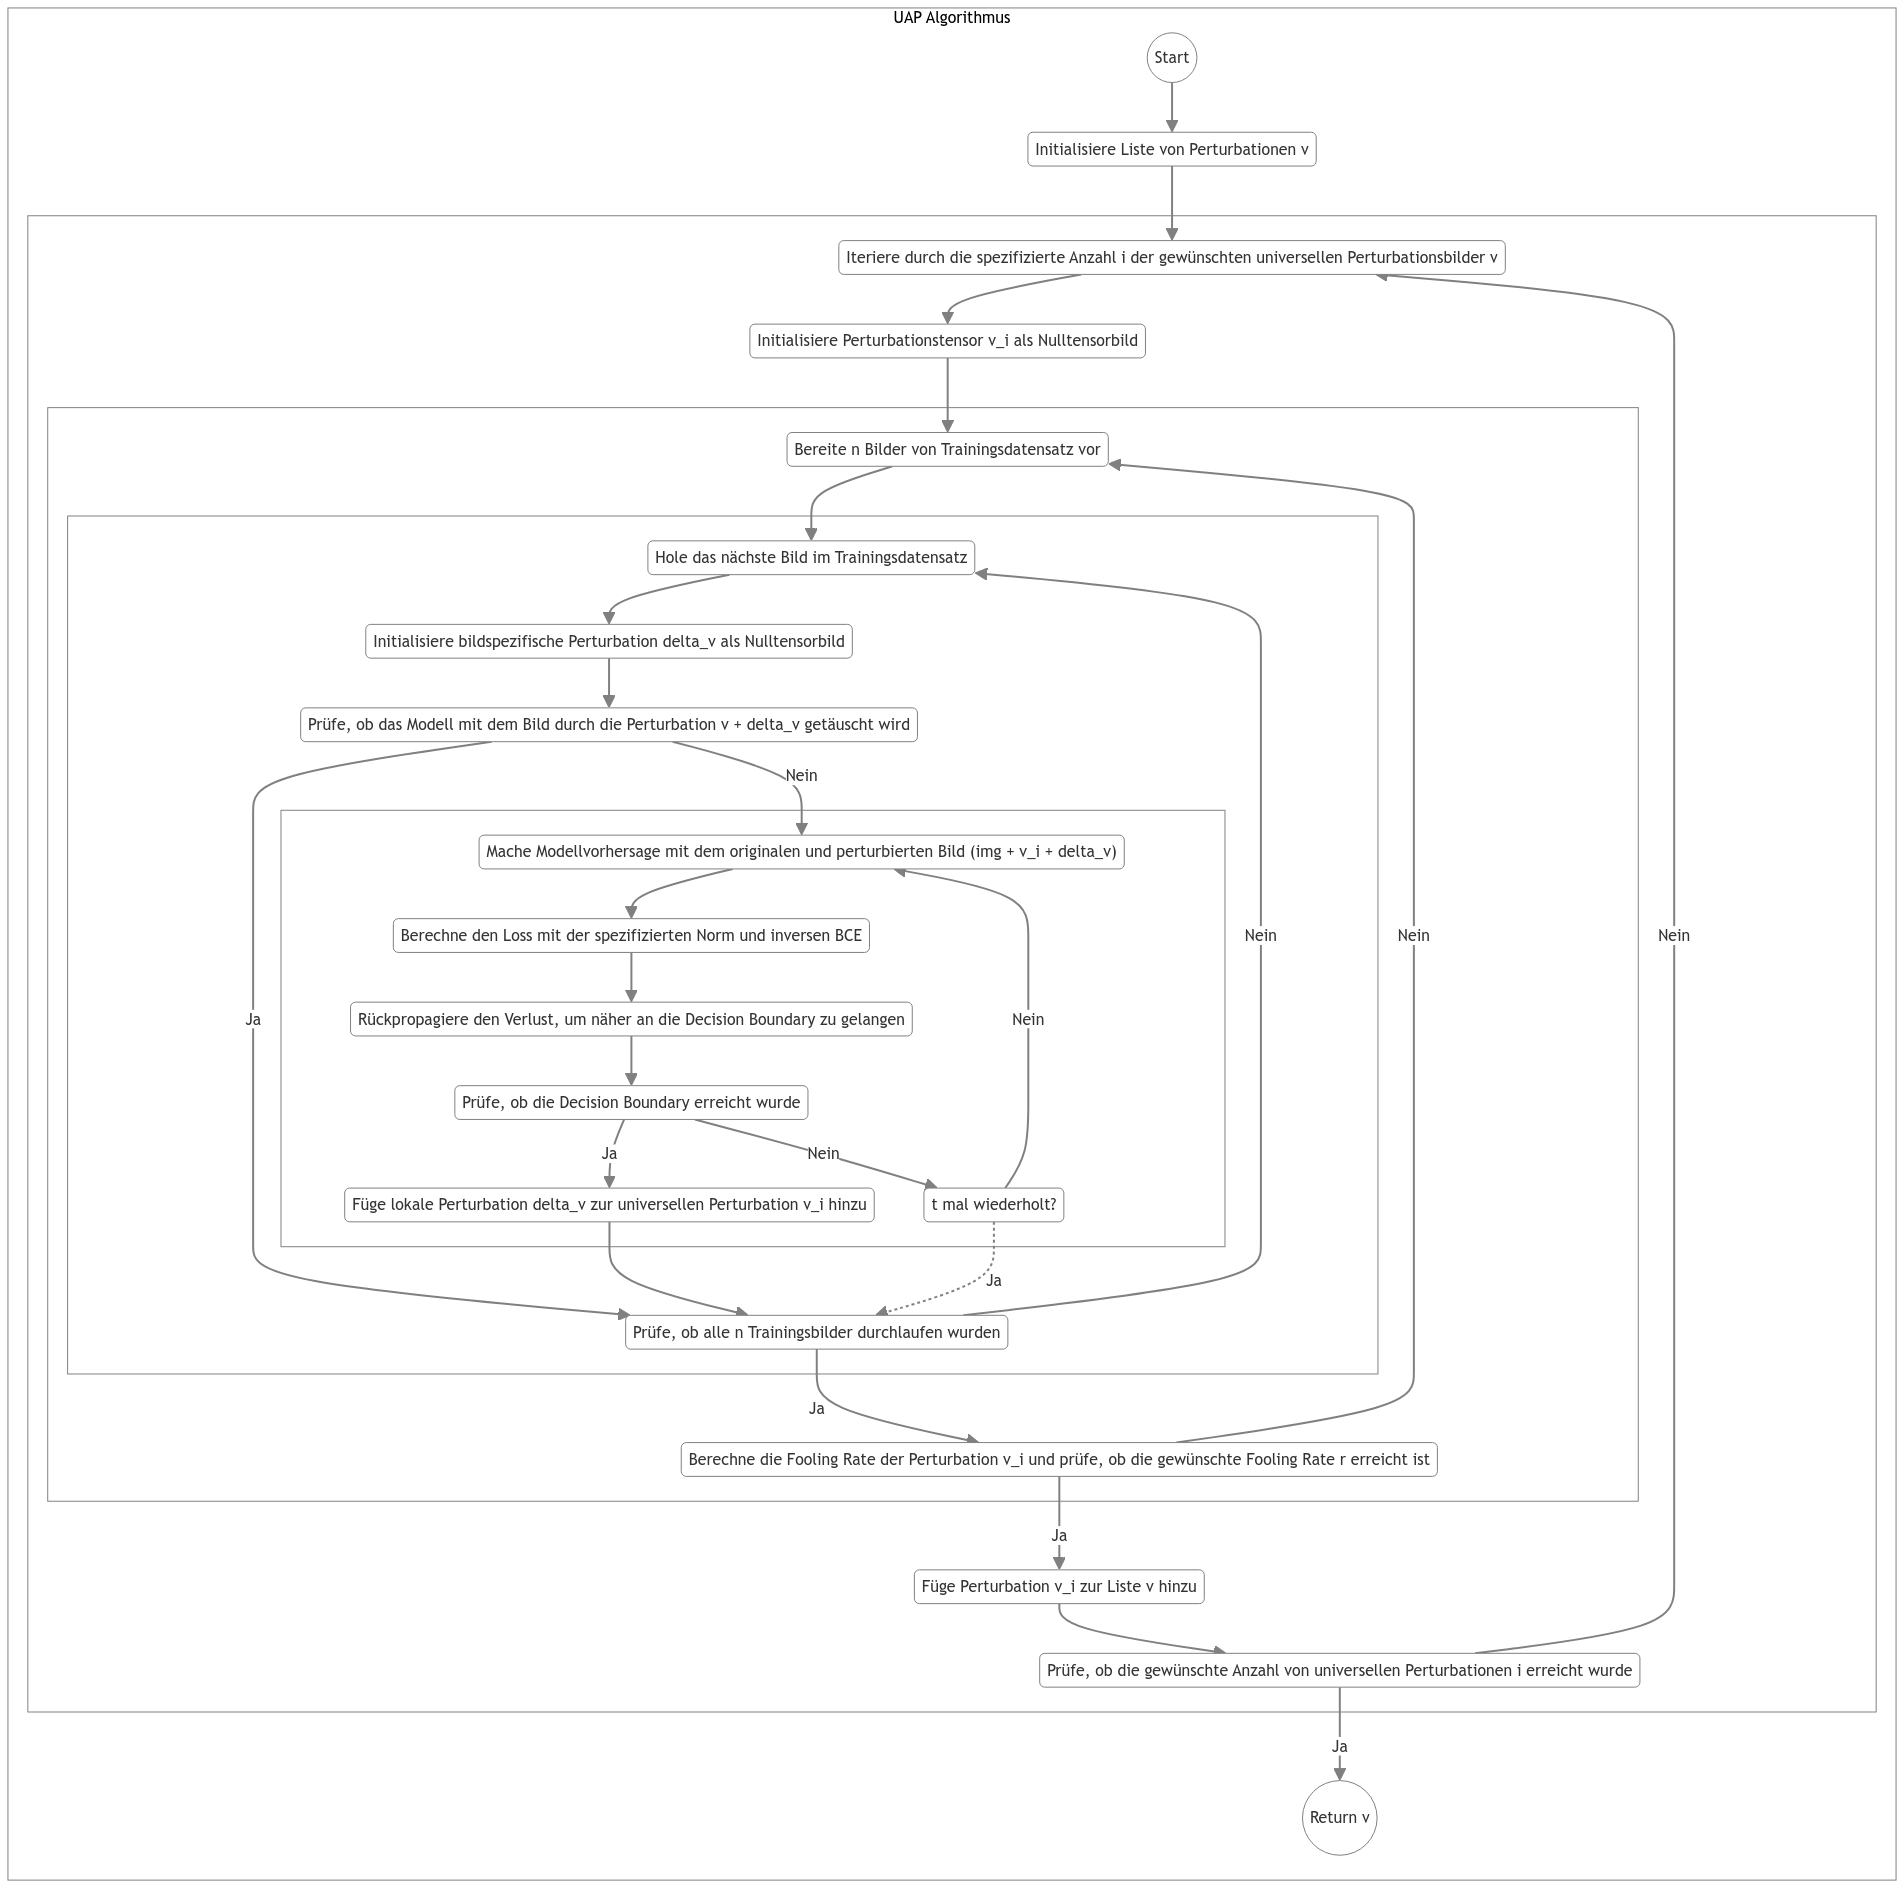
\includegraphics[width=\linewidth]{01-images/04-methodik/UAP_ALG.png}
    \caption{Schematische Darstellung des UAP-Generierungsprozesses}
    \label{fig:05-uap_algorithm}
\end{figure}

\newpage

\subsection*{Technische Umsetzung der Adversarial Training Pipeline}

\todo{Anpassen -> Inferenz auf Test sowie Val}

\begin{algorithm}
\caption{Pipeline zur Generierung von universelle adversarial Perturbationen}
\label{alg:UAP_Adversarial_Training_Pipeline}
\begin{algorithmic}[1]
\STATE Modell $f(\cdot)$ laden
\FOR{Anzahl Robustifizierungen $n_{\text{robustifications}}$}
    \STATE Generierung der \acrshort{uap}s (Algorithmus \ref{algo:UAP Algorithmus})
    \STATE Inferenz auf den Testdaten $X_{\text{test}}$ ($p_{\text{adv}}$=0.0)
    \FOR{jede \acrshort{uap}}
        \STATE Inferenz auf den Testdaten $X_{\text{test}}$ mit \acrshort{uap} ($p_{\text{adv}}$=1.0)
    \ENDFOR
    \STATE Modell finetuning mittels \acrshort{uap}s ($X_{\text{train}}$, $X_{\text{val}}$, random selection, $p_{\text{adv},\text{train}}$=0.5, \\
    $p_{\text{adv},\text{val}}$=0.5)
    \STATE Laden des besten Modellcheckpoints
    \STATE Inferenz auf den Testdaten $X_{\text{test}}$ mit dem robustifiziertem Modell ($p_{\text{adv}}$=0.0)
    \FOR{jede \acrshort{uap}}
        \STATE Inferenz auf den Testdaten $X_{\text{test}}$ mit \acrshort{uap} mit dem robustifizierem Modell ($p_{\text{adv}}$=1.0)
    \ENDFOR
\ENDFOR
\end{algorithmic}
\end{algorithm}

Eine vereinfachte, visualisierte Version der Adversarial Training Pipeline:

\begin{figure}[H]
    \centering
    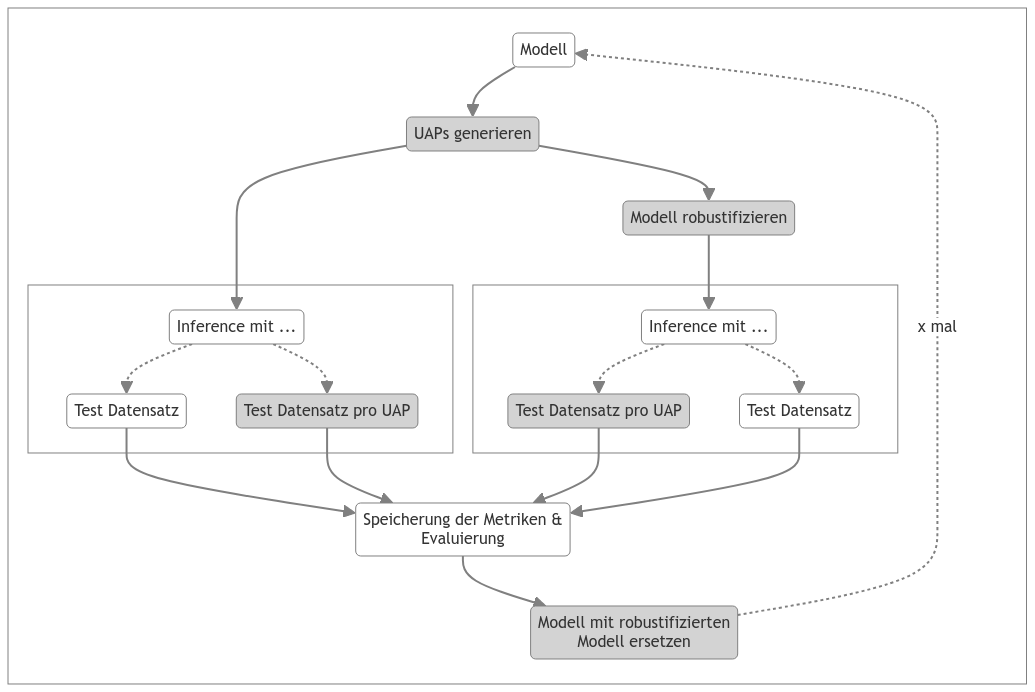
\includegraphics[width=\linewidth]{01-images/04-methodik/robustifizierungs-pipeline.png}
    \caption{Übersicht der Evaluierungspipeline}
    \label{fig:Evaluierungspipeline}
\end{figure}

\newpage

\subsection*{Weitere Analysen}

\subsubsection*{Feature Maps \& PCA} \label{chap:FeatureMaps-TestProblemEda3-mri}

Im Rahmen unserer Analyse nutzen wir ein ResNet50-Modell, das zum einen durch PyTorch vorab trainiert und zum anderen speziell auf unseren Datensatz angepasst. Besonderes Augenmerk liegt auf der Featureextraktion aus dem vorletzten Layer des Modells, direkt vor dem Klassifikationslayer. Die in diesem Schritt gewonnenen Vektoren, auch als Feature Maps bekannt, durchlaufen einer PCA Dimensionsreduktion. Ziel dieser Reduktion ist es, die Dimensionalität der Daten auf zwei Dimensionen zu reduzieren, um eine Visualisierung der verschiedenen Datenpartitionen zu ermöglichen. Die Interpretation erweist sich als sehr komplex und die Ergebnisse sind nur schwer zu interpretieren. 

\paragraph*{Covid}

\begin{figure}[H]
    \centering
    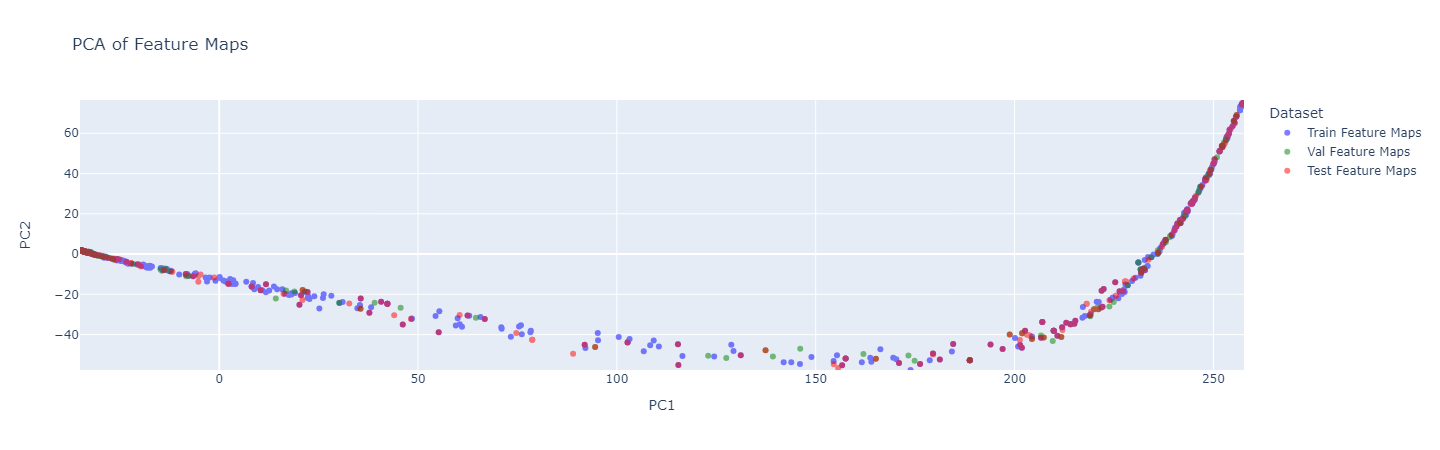
\includegraphics[width=\linewidth]{01-images/06-ending/covidx-all-feautremap-pca-ourmodel-resnet50.png}
    \caption{Hauptkomponenten der PCA-Analyse von zweitletzten Covid Featuremaps Layer eines vortrainierten ResNet50-Modells für Covid}
    \label{fig:covidx-feautremap-pca-ourmodel-resnet50}
\end{figure}

\begin{figure}[H]
    \centering
    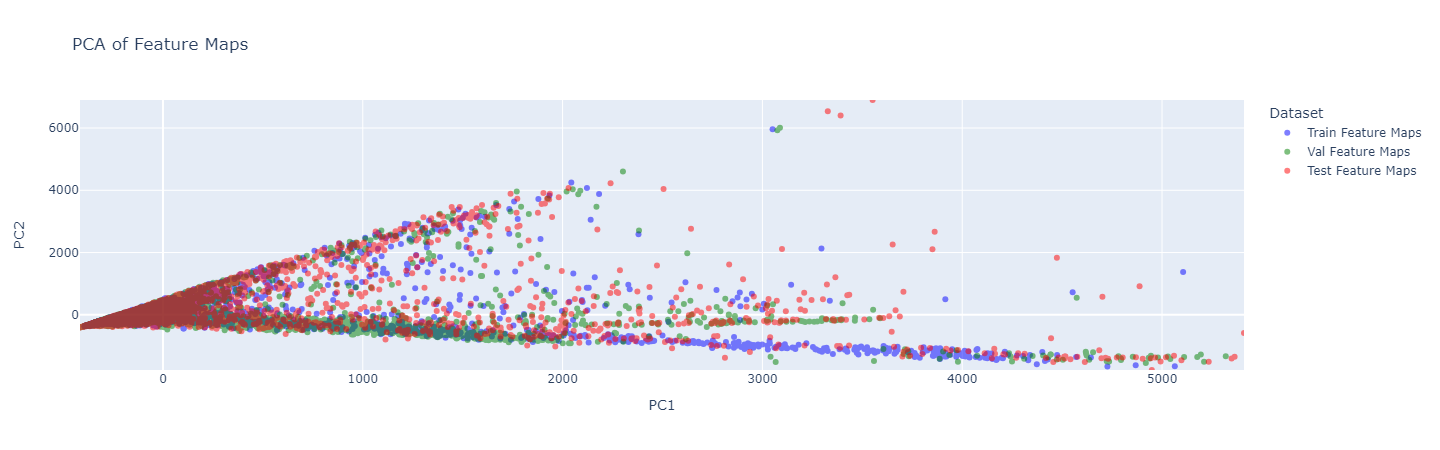
\includegraphics[width=\linewidth]{01-images/06-ending/covidx-all-feautremap-pca-model-resnet50.png}
    \caption{Hauptkomponenten der PCA-Analyse von zweitletzten Covid Featuremaps Layer eines vortrainierten ResNet50-Modells}
    \label{fig:covidx-feautremap-pca-model-resnet50}
\end{figure}


\paragraph*{Hirntumor}

\begin{figure}[H]
    \centering
    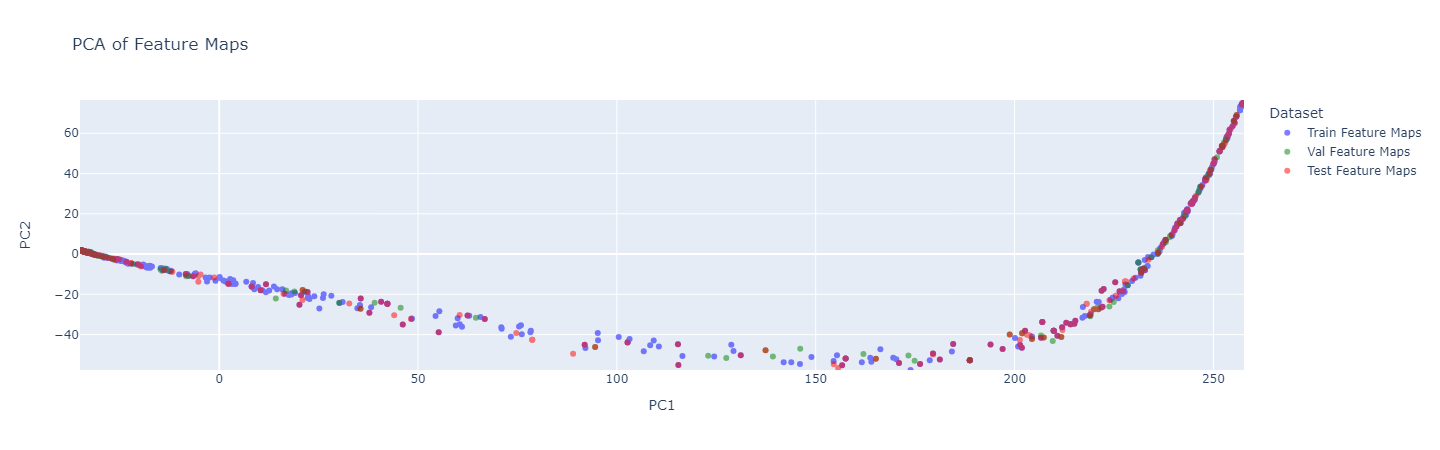
\includegraphics[width=\linewidth]{01-images/06-ending/brain-all-feautremap-pca-ourmodel-resnet50.png}
    \caption{Hauptkomponenten der PCA-Analyse von zweitletzten Hirntumor Featuremaps Layer eines vortrainierten ResNet50-Modells für Hirntumor}
    \label{fig:brain-feautremap-pca-ourmodel-resnet50}
\end{figure}

\begin{figure}[H]
    \centering
    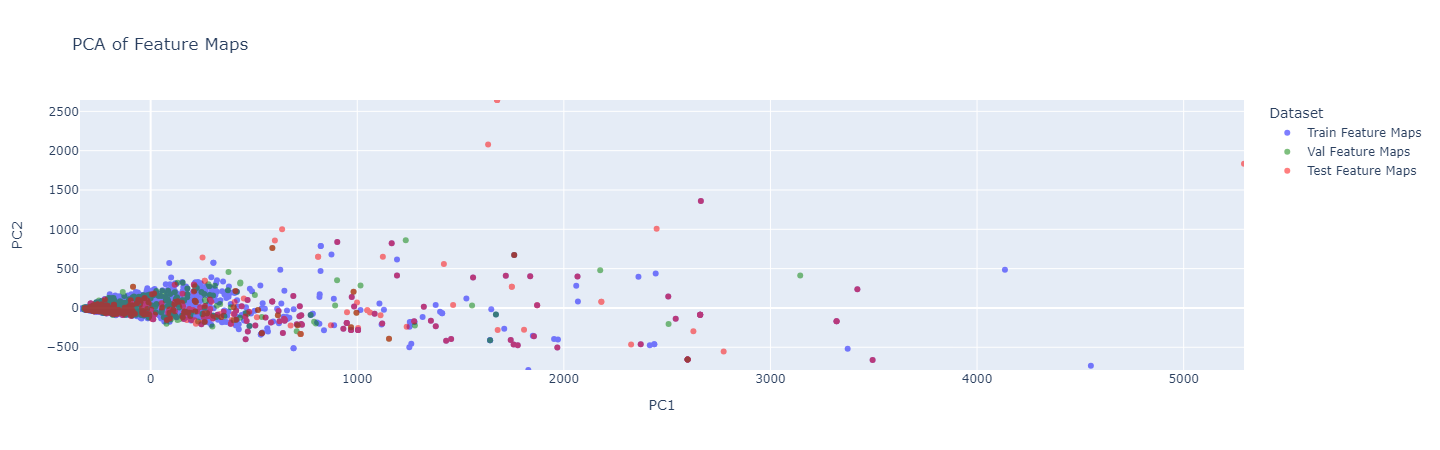
\includegraphics[width=\linewidth]{01-images/06-ending/brain-all-feautremap-pca-model-resnet50.png}
    \caption{Hauptkomponenten der PCA-Analyse von zweitletzten Hirntumor Featuremaps Layer eines vortrainierten ResNet50-Modells}
    \label{fig:brain-feautremap-pca-model-resnet50}
\end{figure}

\newpage

\subsection*{Verlinkungen}

\begin{itemize}

    \item \textbf{GitHub Repositories} \\
    \href{https://github.com/AdversarialAttacks}{https://github.com/AdversarialAttacks}
    
    \item \textbf{Weights \& Bias} \\
    \href{https://wandb.ai/24FS_I4DS27}
    {https://wandb.ai/24FS\_I4DS27}
    
    \item \textbf{UAP Algorithmus} \\
    \href{https://github.com/AdversarialAttacks/report/blob/main/01-images/05-UAP_ALG.png}{UAP Algorithmus}
    
\end{itemize}
